\documentclass[tikz,border=6pt]{standalone}
% Shared style for the model diagrams in this folder.
% Each diagram is a standalone document that inputs this file after
% \documentclass[tikz,border=6pt]{standalone}.
% scripts/build_diagrams.sh compiles every diagram except this file.

\usepackage[T1]{fontenc}
\usepackage[scaled=0.95]{helvet}
\renewcommand{\familydefault}{\sfdefault}
\usepackage{amsmath,amssymb}
\usetikzlibrary{arrows.meta,positioning,fit,backgrounds,calc,shapes.misc}

% Palette: one colour per role.
% Latent quantities are blue, observed data orange, quantities taken from
% the joint fit purple, and parameters a neutral grey.
\definecolor{latentfill}{HTML}{E3EEF9}
\definecolor{latentline}{HTML}{2B5C8A}
\definecolor{datafill}{HTML}{FCE9D6}
\definecolor{dataline}{HTML}{B35A12}
\definecolor{jointfill}{HTML}{EEE4F5}
\definecolor{jointline}{HTML}{6A3D9A}
\definecolor{paramfill}{HTML}{F2F2F2}
\definecolor{paramline}{HTML}{6E6E6E}
\definecolor{textgrey}{HTML}{4A4A4A}

\tikzset{
  every node/.style={font=\small, text=black,
    execute at begin node={\thickmuskip=5mu\medmuskip=4mu\thinmuskip=3mu
      \hyphenpenalty=10000\exhyphenpenalty=10000}},
  box/.style={rectangle, rounded corners=3pt, draw, line width=0.8pt,
    align=center, inner sep=5pt, minimum height=9mm},
  latent/.style={box, fill=latentfill, draw=latentline},
  data/.style={box, fill=datafill, draw=dataline},
  joint/.style={box, fill=jointfill, draw=jointline},
  param/.style={box, fill=paramfill, draw=paramline},
  group/.style={rectangle, rounded corners=6pt, draw=#1, line width=0.8pt,
    dashed, inner sep=8pt},
  grouplabel/.style={font=\small\bfseries, text=#1, anchor=south west,
    inner sep=2pt},
  flow/.style={-{Stealth[length=2.6mm,width=2mm]}, line width=0.9pt,
    draw=black!75},
  jointflow/.style={flow, draw=jointline, line width=1.1pt},
  biflow/.style={{Stealth[length=2.4mm,width=1.9mm]}-{Stealth[length=2.4mm,width=1.9mm]},
    line width=0.9pt, draw=latentline},
  edgelabel/.style={font=\footnotesize, text=textgrey, fill=white,
    inner sep=1.5pt, align=center},
  note/.style={font=\footnotesize, text=textgrey, align=left},
  title/.style={font=\normalsize\bfseries, align=center},
  tag/.style={rectangle, rounded corners=2pt, fill=jointline,
    text=white, font=\scriptsize\bfseries, inner sep=2pt},
}


% The health-zone model and how the joint fit enters it. The zone model
% runs top to bottom on the left. Each purple box on the right is an input
% from the joint fit, level with the step it feeds and badged by how it
% enters: sampled through the meld, fixed at a posterior mean, or used to
% fit a prior. Purple symbols inside the zone boxes come from the joint fit.

\newcommand{\J}[1]{{\color{jointline}#1}}

\begin{document}
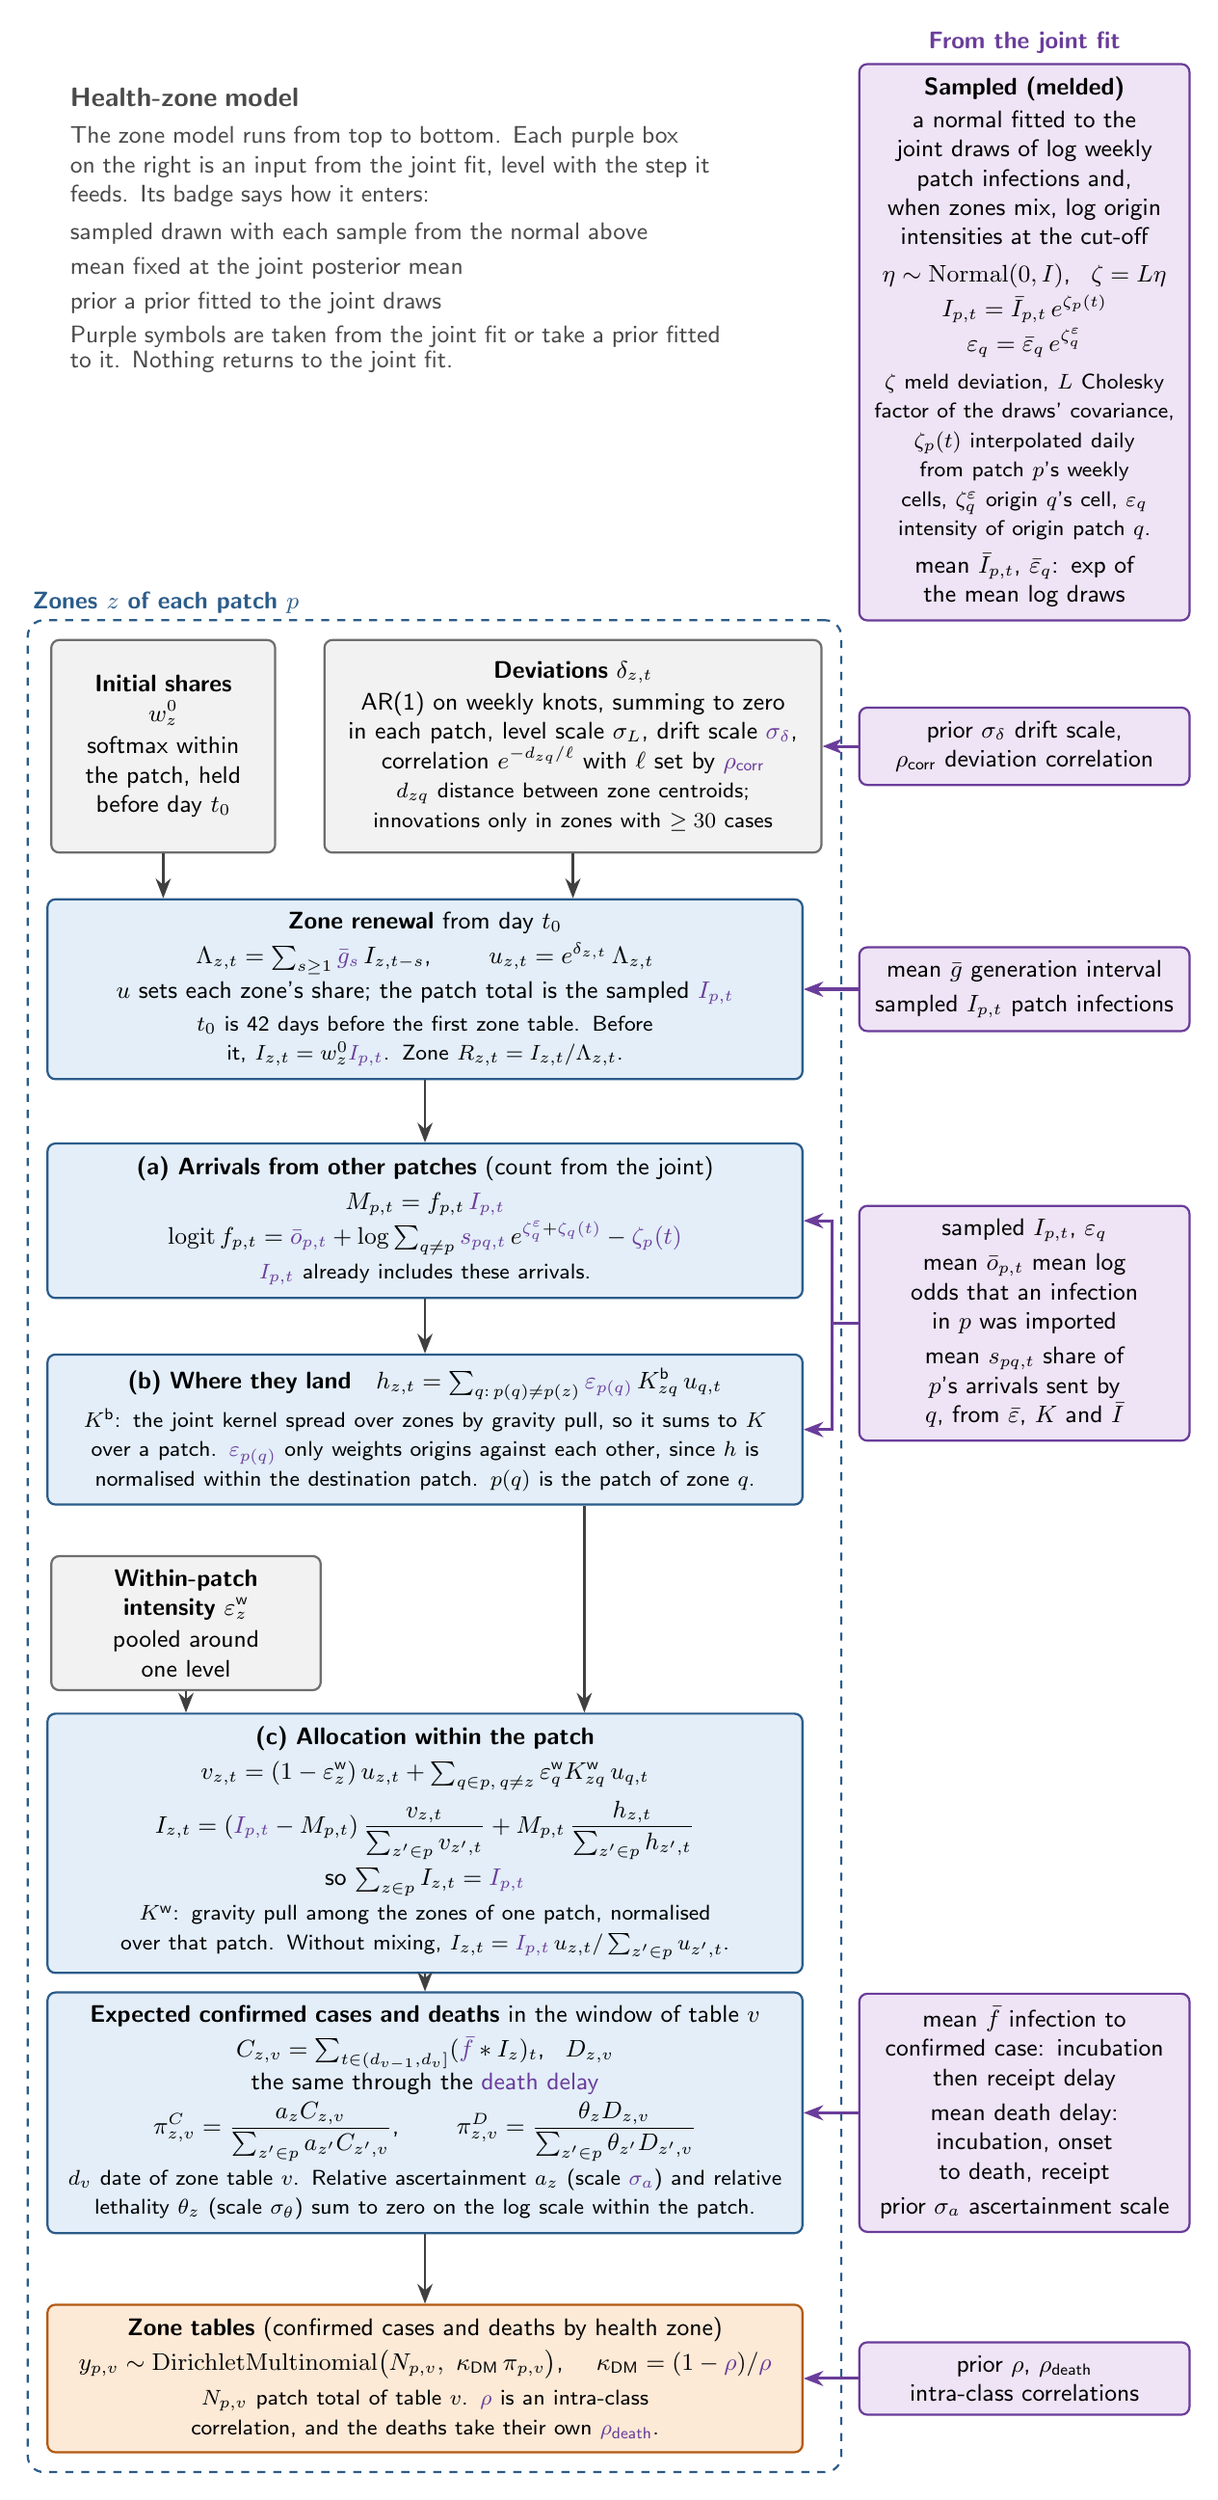
\begin{tikzpicture}[x=1cm,y=1cm]

\def\xs{-2.6}     % zone stack centre
\def\ws{9.6cm}    % zone stack text width
\def\xj{5.3}      % joint input column centre
\def\wj{4.0cm}    % joint input text width

% ---- Sampled (melded) box at the top of the input column --------------------
\node[grouplabel=jointline, anchor=south] at (\xj,0.05) {From the joint fit};
\node[joint, text width=\wj, anchor=north] (meld) at (\xj,0)
  {\textbf{Sampled (melded)}\\[1pt]
   a normal fitted to the joint draws of log weekly patch infections and,
   when zones mix, log origin intensities at the cut-off\\[3pt]
   $\eta \sim \mathrm{Normal}(0, I)$, \enspace $\zeta = L\eta$\\[2pt]
   $I_{p,t} = \bar I_{p,t}\, e^{\zeta_p(t)}$\\[2pt]
   $\varepsilon_q = \bar\varepsilon_q\, e^{\zeta^{\varepsilon}_q}$\\[3pt]
   {\footnotesize $\zeta$ meld deviation, $L$ Cholesky factor of the draws'
   covariance, $\zeta_p(t)$ interpolated daily from patch $p$'s weekly cells,
   $\zeta^{\varepsilon}_q$ origin $q$'s cell, $\varepsilon_q$ intensity of
   origin patch $q$.}\\[3pt]
   \badge{mean} $\bar I_{p,t}$, $\bar\varepsilon_q$: exp of the mean log draws};

\node[note, text width=8.6cm, anchor=north west] (intro) at (-7.4,-0.2)
  {\normalsize\textbf{Health-zone model}\\[3pt]
   \small The zone model runs from top to bottom.
   Each purple box on the right is an input from the joint fit, level with
   the step it feeds. Its badge says how it enters:\\[3pt]
   \badge{sampled} drawn with each sample from the normal above\\[2pt]
   \badge{mean} fixed at the joint posterior mean\\[2pt]
   \badge{prior} a prior fitted to the joint draws\\[3pt]
   Purple symbols are taken from the joint fit or take a prior fitted to it.
   Nothing returns to the joint fit.};

% ---- Zone stack ---------------------------------------------------------------
\def\yP{-9.0}
\node[param, text width=2.6cm, minimum height=28mm] (w0) at (-6.05,\yP)
  {\textbf{Initial shares}\\ $w^0_z$\\[1pt] softmax within the patch, held before day $t_0$};
\node[param, text width=6.2cm, minimum height=28mm] (dev) at (-0.65,\yP)
  {\textbf{Deviations} $\delta_{z,t}$\\[1pt]
   AR(1) on weekly knots, summing to zero\\ in each patch,
   level scale $\sigma_L$, drift scale $\J{\sigma_\delta}$,\\
   correlation $e^{-d_{zq}/\ell}$ with $\ell$ set by $\J{\rho_{\text{corr}}}$\\
   {\footnotesize $d_{zq}$ distance between zone centroids;}\\
   {\footnotesize innovations only in zones with $\ge 30$ cases}};

\node[latent, text width=\ws] (ren) at (\xs,-12.2)
  {\textbf{Zone renewal} from day $t_0$\\[2pt]
   $\Lambda_{z,t} = \sum_{s \ge 1} \J{\bar g_s}\, I_{z,t-s}$, \qquad
   $u_{z,t} = e^{\delta_{z,t}}\, \Lambda_{z,t}$\\[2pt]
   $u$ sets each zone's share; the patch total is the sampled $\J{I_{p,t}}$\\[1pt]
   {\footnotesize $t_0$ is 42 days before the first zone table. Before it,
   $I_{z,t} = w^0_z \J{I_{p,t}}$. Zone $R_{z,t} = I_{z,t} / \Lambda_{z,t}$.}};

\node[latent, text width=\ws] (arr) at (\xs,-15.25)
  {\textbf{(a) Arrivals from other patches} (count from the joint)\\[2pt]
   $M_{p,t} = f_{p,t}\, \J{I_{p,t}}$\\[2pt]
   $\operatorname{logit} f_{p,t} = \J{\bar o_{p,t}}
     + \log \sum_{q \ne p} \J{s_{pq,t}}\, e^{\J{\zeta^{\varepsilon}_q} + \J{\zeta_q(t)}}
     - \J{\zeta_p(t)}$\\[2pt]
   {\footnotesize $\J{I_{p,t}}$ already includes these arrivals.}};

\node[latent, text width=\ws] (land) at (\xs,-18.0)
  {\textbf{(b) Where they land}\quad
   $h_{z,t} = \sum_{q:\, p(q) \ne p(z)} \J{\varepsilon_{p(q)}}\, K^{\text{b}}_{zq}\, u_{q,t}$\\[2pt]
   {\footnotesize $K^{\text{b}}$: the joint kernel spread over zones by gravity
   pull, so it sums to $K$ over a patch. $\J{\varepsilon_{p(q)}}$ only weights
   origins against each other, since $h$ is normalised within the destination
   patch. $p(q)$ is the patch of zone $q$.}};

\node[param, text width=3.2cm] (epsw) at (-5.75,-20.55)
  {\textbf{Within-patch}\\ \textbf{intensity} $\varepsilon^{\text{w}}_z$\\[1pt]
   pooled around one level};

\node[latent, text width=\ws] (alloc) at (\xs,-23.45)
  {\textbf{(c) Allocation within the patch}\\[2pt]
   $v_{z,t} = (1 - \varepsilon^{\text{w}}_z)\, u_{z,t}
     + \sum_{q \in p,\, q \ne z} \varepsilon^{\text{w}}_q K^{\text{w}}_{zq}\, u_{q,t}$\\[3pt]
   $I_{z,t} = (\J{I_{p,t}} - M_{p,t})\,
     \dfrac{v_{z,t}}{\sum_{z' \in p} v_{z',t}}
     + M_{p,t}\, \dfrac{h_{z,t}}{\sum_{z' \in p} h_{z',t}}$\\[2pt]
   so $\sum_{z \in p} I_{z,t} = \J{I_{p,t}}$\\[2pt]
   {\footnotesize $K^{\text{w}}$: gravity pull among the zones of one patch,
   normalised over that patch.
   Without mixing, $I_{z,t} = \J{I_{p,t}}\, u_{z,t} / \sum_{z' \in p} u_{z',t}$.}};

\node[latent, text width=\ws] (exc) at (\xs,-27.0)
  {\textbf{Expected confirmed cases and deaths} in the window of table $v$\\[2pt]
   $C_{z,v} = \sum_{t \in (d_{v-1}, d_v]} (\J{\bar f} * I_z)_t$, \enspace
   $D_{z,v}$ the same through the \J{death delay}\\[2pt]
   $\pi^{C}_{z,v} = \dfrac{a_z C_{z,v}}{\sum_{z' \in p} a_{z'} C_{z',v}}$, \qquad
   $\pi^{D}_{z,v} = \dfrac{\theta_z D_{z,v}}{\sum_{z' \in p} \theta_{z'} D_{z',v}}$\\[2pt]
   {\footnotesize $d_v$ date of zone table $v$. Relative ascertainment $a_z$
   (scale $\J{\sigma_a}$) and relative lethality $\theta_z$ (scale $\sigma_\theta$)
   sum to zero on the log scale within the patch.}};

\node[data, text width=\ws] (obs) at (\xs,-30.5)
  {\textbf{Zone tables} (confirmed cases and deaths by health zone)\\[2pt]
   $y_{p,v} \sim \mathrm{DirichletMultinomial}\bigl(N_{p,v},\ \kappa_{\text{DM}}\, \pi_{p,v}\bigr)$,
   \quad $\kappa_{\text{DM}} = (1 - \J{\rho}) / \J{\rho}$\\[2pt]
   {\footnotesize $N_{p,v}$ patch total of table $v$. $\J{\rho}$ is an
   intra-class correlation, and the deaths take their own $\J{\rho_{\text{death}}}$.}};

% Zone flow.
\draw[flow] (w0.south) -- (w0.south |- ren.north);
\draw[flow] (dev.south) -- (dev.south |- ren.north);
\draw[flow] (ren) -- (arr);
\draw[flow] (arr) -- (land);
\draw[flow] (land.south -| -0.5,0) -- (-0.5,0 |- alloc.north);
\draw[flow] (epsw.south) -- (epsw.south |- alloc.north);
\draw[flow] (alloc) -- (exc);
\draw[flow] (exc) -- (obs);

\begin{scope}[on background layer]
  \node[group=latentline, fit=(w0) (dev) (obs), inner sep=7pt] (zgrp) {};
\end{scope}
\node[grouplabel=latentline] at (zgrp.north west) {Zones $z$ of each patch $p$};

% ---- Joint inputs, level with the step each feeds ---------------------------
\node[joint, text width=\wj] (j1) at (\xj,\yP)
  {\badge{prior} $\sigma_\delta$ drift scale,\\ $\rho_{\text{corr}}$ deviation correlation};
\node[joint, text width=\wj] (j2) at (\xj,-12.2)
  {\badge{mean} $\bar g$ generation interval\\[2pt]
   \badge{sampled} $I_{p,t}$ patch infections};
\node[joint, text width=\wj] (j3) at (\xj,-16.6)
  {\badge{sampled} $I_{p,t}$, $\varepsilon_q$\\[2pt]
   \badge{mean} $\bar o_{p,t}$ mean log odds that an infection in $p$ was imported\\[2pt]
   \badge{mean} $s_{pq,t}$ share of $p$'s arrivals sent by $q$, from $\bar\varepsilon$,
   $K$ and $\bar I$};
\node[joint, text width=\wj] (j5) at (\xj,-27.0)
  {\badge{mean} $\bar f$ infection to confirmed case: incubation then receipt delay\\[2pt]
   \badge{mean} death delay: incubation, onset to death, receipt\\[2pt]
   \badge{prior} $\sigma_a$ ascertainment scale};
\node[joint, text width=\wj] (j6) at (\xj,-30.5)
  {\badge{prior} $\rho$, $\rho_{\text{death}}$\\ intra-class correlations};

\draw[jointflow] (j1.west) -- (dev.east);
\draw[jointflow] (j2.west) -- (ren.east |- j2.west);
\draw[jointflow] (j3.west) -- ++(-0.35,0) |- (arr.east);
\draw[jointflow] (j3.west) -- ++(-0.35,0) |- (land.east);
\draw[jointflow] (j5.west) -- (exc.east |- j5.west);
\draw[jointflow] (j6.west) -- (obs.east |- j6.west);

% ---- Key -------------------------------------------------------------------
\colourkey[joint]{(-7.4,-33.0)}

\end{tikzpicture}
\end{document}
